\chapter{Asking a Private Equity Millionaire How He Got Rich}

This chapter follows a School of Hard Knocks interview that is not mathematical on its surface, yet is highly structured beneath the surface. We are taken from a viral claim about private equity into a series of practical questions about career formation, capital allocation, industry choice, sales structure, family life, habits, solitude, recovery after loss, and legacy. The notes below keep the order and motive of that unfolding intact. Where the interview speaks in plain commercial language, we allow ourselves a cautious companion mathematics, not to overwrite the speaker, but to make the hidden logic easier to see.

\begin{remark}
No validated board equations or diagram screenshots survive for this chapter. Every displayed formula below is therefore an editorial reconstruction from the transcript. We use notation only when it clarifies a mechanism that the speaker is plainly describing.
\end{remark}

\section{Opening Hook and an Uneven Beginning}

The hosts do not introduce Mike Kessner as an abstract expert. They re-enter through an old and very public claim. A previous clip had gone viral because Mike had answered a blunt question --- what industry is best for getting wealthy? --- with the answer: private equity. The new interview begins by reopening that old answer and then adding a strange, almost comic update: his son later moved from consulting into a large private-equity firm, while his son-in-law moved from investment banking into a private-equity venture of his own. The point is not causation. The point is that judgments about where wealth accumulates tend to echo outward.

From there the hosts do the right thing. They ask for the path. Mike gives them a path that is not at all tidy: LSU, an unrealized baseball ambition, a transfer to Denver, a first job in recruiting that ended after roughly a month, then a move through a large company and eventually into insurance, where he stayed for over thirty years. The story matters precisely because it is uneven. The interview is quietly stripping away the myth that a successful commercial life begins from a polished starting point.

\begin{definition}
Let \(C_t\) denote \emph{career capital} at time \(t\). By this we mean the accumulated stock of competence, credibility, relationships, position, and repeatable execution that makes later opportunities easier to capture.
\end{definition}

A useful companion model is
\begin{equation}
C_{t+1}=C_t+\alpha S_t+\beta N_t+\gamma R_t+\delta E_t,
\end{equation}
where \(S_t\) is skill, \(N_t\) is network quality, \(R_t\) is reputation, and \(E_t\) is execution. The speaker never writes this down, but he describes exactly this sort of process. For the first several years in insurance, he says, he did not really know what he was doing. What he did know was that authentic, high-energy people tend, over time, to become successful; if he stayed near them and kept working, that current would do some of the work.

If we iterate the update rule, we get
\begin{align}
C_n-C_0
&=\sum_{t=0}^{n-1}\bigl(\alpha S_t+\beta N_t+\gamma R_t+\delta E_t\bigr).
\end{align}
This is the right place to pause. The interview is not claiming that one brilliant year explains the whole later outcome. It is claiming something slower and more consequential: if the terms on the right-hand side remain positive over a long interval, then the later outcome will look sudden only to people who did not watch the accumulation.

The speaker's own verbal version can be written more compactly as
\begin{equation}
N_t \uparrow \text{ through authentic, high-energy people}
\Longrightarrow
\Pr(\text{future success}\mid t)\uparrow.
\end{equation}
This is the first deep commercial proposition in the chapter. It says that who we stand near is not merely social decoration. It is one of the state variables.

The story then advances in the same measured way. Mike spends roughly twenty-five years in that long game, meets a younger CEO in the insurance world, imagines at first that his old firm might eventually acquire the younger man's company, and instead finds himself drawn into a new phase. His old firm had become a large private-equity roll-up of about two thousand people. The newer phase, by his account, has been the most enjoyable part of the career, because the objective has widened. It is no longer only about personal earnings; it is about coaching younger people and leaving behind something of value.

\section{Wealth, Timing, and the New Industry Question}

Once the career path has been laid out, the hosts shift very naturally to capital allocation. The move is important. Biography alone does not tell us how a person thinks under uncertainty. Best and worst financial decisions do.

A minimal wealth equation is
\begin{equation}
W_{t+1}=W_t+Y_t+\Pi_t-L_t,
\end{equation}
where \(W_t\) is the stock of wealth, \(Y_t\) is earned income, \(\Pi_t\) is investment profit or loss, and \(L_t\) is the outflow required to live. In the interview, \(\Pi_t\) is immediately decomposed into cases:
\begin{equation}
\Pi_t=\Pi_t^{\text{Nautilus}}+\Pi_t^{\text{Coinbase}}+\Pi_t^{\text{home}}+\cdots.
\end{equation}

Nautilus is the favorable case. Mike reads about the company shortly before the pandemic, recognizes the home-fitness angle, adds capital, and then benefits from a massive shift in consumer behavior. He calls the outcome luck, and the notes should preserve that humility. The decision contains alertness and timing, but no false theorem of omniscience.

Coinbase becomes the obvious losing case, though one he still holds. The family home is subtler. Financially, it produced almost no gain over a period of about twenty years. Yet Mike refuses to call it a bad decision in any simple sense, because it housed a family, a neighborhood, and a long set of memories. The interview thereby introduces a distinction that good notes should not flatten away: a position may disappoint as \(\Pi_t\) and still be indispensable in the larger accounting of a life.

\begin{remark}
This is one place where we should resist the temptation to compress everything into a single scalar objective. The interview plainly distinguishes financial return from lived return.
\end{remark}

At exactly this point, the hosts ``circle back'' to the earlier viral question. What industry should young people be looking at now? Mike updates the answer. He says data science; more broadly, analytics. He is careful not to posture as the technical expert. Instead he explains the value of analytics from the inside of a real firm. The younger analytic talent crunches data, identifies what is trending, and brings those signals to more experienced operators.

A natural schematic is
\begin{equation}
D \rightarrow A \rightarrow Z \rightarrow \text{decision},
\end{equation}
where \(D\) is raw data, \(A\) is the analytics layer, and \(Z\) is the extracted signal about what is changing. Mike compares the process to ``Moneyball,'' and the comparison is exact. We are not merely collecting facts; we are building an information pipeline that changes where managerial attention lands. This is why analytics matters. It sharpens selection.

\subsection{Question \& Answer}

\paragraph{Question.} Why does the interview move from stocks and career choices to data science and analytics?

\paragraph{Answer.} Because the real question is not only where wealth has been, but how a firm learns where value is moving. The Nautilus story is about timing under change; the analytics answer generalizes that instinct. A firm that can detect emerging patterns earlier can allocate people, capital, and attention more intelligently. The move into data science is therefore not a fad answer. It is an answer about information leverage.

\section{From Analytics to Sales Architecture}

Before changing topics, the hosts stay with insurance long enough to ask a much better question than ``Is insurance good?'' They ask what structure inside insurance gives a young person a real chance.

Mike answers first by negation: sales is lonely when it is done on an island. This is one of the interview's cleanest lines, because it does not merely describe an emotion. It diagnoses a defective organizational form. The speaker wants young people entering insurance, and then more generally anyone entering sales, to land in a team environment that feels less like solitary commission chasing and more like a functioning sports culture. The transcript is noisy around the repeated ``make it like sports'' phrasing, but the argument itself is clear.

To make that argument crisp, let
\begin{equation}
Q_{\text{sales}}=f(G,V,M),
\end{equation}
where \(Q_{\text{sales}}\) is the effectiveness of the sales operation, \(G\) is group cohesion, \(V\) is vertical specialization, and \(M\) is the morale and shared learning that come from collective work. The point is not that these variables are measurable to the second decimal place. The point is that the speaker is describing a production function, and it is not the production function of an isolated generalist.

He then explains the structure at his current firm. There are roughly twenty-five sales people, divided across five or six teams with distinct verticals. Private equity is one vertical. Hospitality is another. Construction is another. Restaurants are another, with roughly eight hundred restaurants insured. The internal advantage of the firm is that it can send people into these worlds who already know how those worlds speak.

\subsection{Question \& Answer}

\paragraph{Question.} Why should team specialization outperform the strong lone generalist?

\paragraph{Answer.} Because the gain appears twice. First, a real team changes the emotional and learning environment. Winning can be celebrated, losing can be processed, and the knowledge generated in one case can be carried into another. Second, specialization changes the content of the commercial conversation. The seller is no longer generic. He can enter a client's world already fluent in its language, its pain points, and the kinds of solutions that have worked for comparable firms.

We can summarize the second point as
\begin{equation}
V \uparrow \Longrightarrow \text{domain fluency} \uparrow \Longrightarrow \text{client trust} \uparrow.
\end{equation}
And once trust rises, the space of possible solutions rises with it. The seller can mention precedents, recurring operational bottlenecks, and better alternatives without sounding like an outsider trying to improvise expertise.

\begin{figure}
\centering
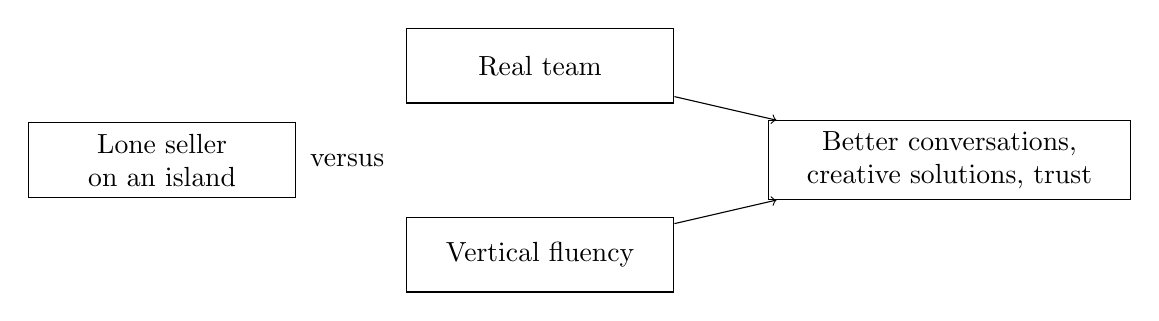
\begin{tikzpicture}[x=1cm,y=1cm]
\node[draw, rectangle, minimum width=3.4cm, minimum height=0.95cm, align=center] (a) at (0,0) {Lone seller\\on an island};
\node[draw, rectangle, minimum width=3.4cm, minimum height=0.95cm, align=center] (b) at (4.8,1.2) {Real team};
\node[draw, rectangle, minimum width=3.4cm, minimum height=0.95cm, align=center] (c) at (4.8,-1.2) {Vertical fluency};
\node[draw, rectangle, minimum width=4.6cm, minimum height=1cm, align=center] (d) at (10,0) {Better conversations,\\creative solutions, trust};
\node at (2.35,0) {versus};
\draw[->] (b) -- (d);
\draw[->] (c) -- (d);
\end{tikzpicture}
\end{figure}

This diagram is editorial, but its logic is fully transcript-backed. The interview's real lesson is that edge does not come from a mystical ``sales secret.'' It comes from a better sales architecture.

\section{Temperament, Family, and Daily Habits}

Only after this machinery of work has been established does the interview pivot. The hosts explicitly mark the turn: they have talked about career a great deal and now want to move toward family. Before that move, however, there is a brief and revealing detour through temperament. Asked for the most impactful book in his life, Mike chooses \textit{Don't Sweat the Small Stuff}. He reads or listens to three to five books a month, so the choice is not casual. He could have reached for something grander. Instead he chooses a book whose central lesson is scale: most disturbances are not large enough to deserve panic.

That gives us the right emotional bridge into the family segment. The fatherhood advice is simple but severe: quantity of time with children matters. The small child should know that the parent is there. The marriage advice is equally concrete. If work has been hard, the transition home may need to be deliberate. Pull over. Take a breath. Do not drag the entire office through the front door.

The transcript becomes garbled for a stretch after this, but the underlying line of thought is still recoverable. Mike stresses affection toward spouse and children, even if he is not, by his own description, naturally affectionate with most people. He stresses humor where humor is natural, seriousness where seriousness is required, and common interests as the bridge by which relationship becomes durable. Reading trips with a son, shopping trips with a daughter: the details matter because they make family life specific rather than abstract.

From there the hosts ask about daily habits. Mike answers with a ritual rather than an achievement story: a triple espresso, a short period of meditation, and a brief period of gratitude. The remarkable thing is how modestly he describes the practice. He does not claim mystical emptiness of mind. Much of the time, he says, thoughts of business and family intrude. Yet the practice still works.

\subsection{Question \& Answer}

\paragraph{Question.} Is meditation and gratitude merely soft talk, or do they have operational value?

\paragraph{Answer.} The interview answers this without grand theory. Mike says, with some humor, that the espresso may be the best part. Gratitude, he says, is fairly easy: everyone has something for which to be thankful. Meditation is not pure concentration for him, but a repeated habit that leaves him in a better condition to begin the day. The point is not spiritual exhibition. The point is state preparation.

We may summarize the habit-chain in prose:
\begin{enumerate}
\item start from a fixed ritual;
\item let the ritual lower noise and stabilize attention;
\item begin the workday from a better internal state;
\item repeat this over years rather than days.
\end{enumerate}
This is enough. The interview does not ask us to deify the practice. It asks us to notice that reliable habits alter the initial conditions of the day.

\section{Mindset, Success, and the Use of Solitude}

Once the daily operating system has been laid down, the hosts ask a more abstract question: what mindset change is necessary for someone who wants to become a multimillionaire? Mike's answer is terse, but it is the nearest thing in the interview to a general formula:
\begin{equation}
\text{success}=\text{plan}+\text{tenacity}+\text{execution}.
\end{equation}
This is not literal algebra. It is an order of dependence. A plan without endurance is inert. Endurance without a plan is blind. Execution is what turns both into a real outcome. Mike's emphasis is that many people never really form a plan, or else they give up a day, a week, or a month before the business would have broken through.

The hosts then ask what drives him personally. The answer changes with age. At first the goal was to make a living. Then it was to become more successful and provide more for the family. Now, in what he calls a ``second mountain,'' the goal is legacy. He and his partner entered Virtus about three and a half years ago; by his account the firm has quadrupled in about three years. What matters to him now is not only the firm's growth, but the chance to have a real effect on younger people whose own earning lives are still in front of them.

That leads naturally to the interview's formal definition of success. Mike ranks the goods rather than blending them:
\begin{equation}
U_{\text{family}} \succ U_{\text{freedom}} \succ U_{\text{friends}}.
\end{equation}
Family life comes first. Financial freedom comes next. Then a small number of good friends. This ranking is important because it explains why financial freedom matters without making it supreme. Money is not the summit; it is the thing that lets one breathe, leave bad environments, and act without panic.

His three guiding principles for the next generation then appear as a compact triad:
\begin{equation}
\{\text{work hard},\ \text{be a good teammate},\ \text{spend time alone}\}.
\end{equation}
The first two principles are already familiar from earlier parts of the interview. The third is the surprising one, and the hosts rightly stop to ask why.

\subsection{Question \& Answer}

\paragraph{Question.} Why is alone time a strategic tool rather than a retreat from life?

\paragraph{Answer.} The hosts put the tension clearly: many people are afraid of being alone, afraid of loneliness. Mike's answer is sober rather than romantic. Alone time removes noise. It gets one away from the phone, the computer, and the pressure field in which every local problem presents itself as urgent. Once that noise falls, reflection becomes possible; once reflection becomes possible, planning becomes possible; and once planning becomes possible, non-obvious solutions have a chance to arrive.

That logic can be written as a simple cascade:
\begin{equation}
\text{less noise} \Longrightarrow \text{more reflection}
\Longrightarrow \text{better planning}
\Longrightarrow \text{better decisions}.
\end{equation}
His example is practical and businesslike: leaders in the firm intentionally step away in order to reflect on the year and plan the next one; in one case a CEO goes away alone for several hours to think. Solitude here is not withdrawal. It is an operating condition for judgment.

\section{Restarting from Zero, Building Again, and Leaving Something Behind}

The lecture's most vivid stress test arrives late: if the bank account hit zero tomorrow, what would be the first move? Mike does not offer a cinematic answer. He offers an engine. He would go back into full-time sales because he believes he can still out-hustle and outwork people and generate commission checks quickly. That answer is faithful to the whole interview. When forced to start again, he does not begin with ideology. He begins with cash flow.

A worked companion model is therefore appropriate. We start from
\begin{align}
W_0 &= 0,\\
Y_1 &= Y_1^{\text{sales}}.
\end{align}
The first task is to restore earnings. Only then does allocation become meaningful. Suppose fractions of the first successful sales income are directed into several asset buckets:
\begin{align}
K_1^{\text{RE}} &= \lambda_{\text{RE}}\,Y_1^{\text{sales}},\\
K_1^{\text{PE}} &= \lambda_{\text{PE}}\,Y_1^{\text{sales}},\\
K_1^{\text{hobby}} &= \lambda_{\text{hobby}}\,Y_1^{\text{sales}},
\end{align}
with
\begin{equation}
\lambda_{\text{RE}}+\lambda_{\text{PE}}+\lambda_{\text{hobby}}\le 1.
\end{equation}
The unallocated remainder stays liquid. On the next step, wealth is no longer rebuilt by wages alone:
\begin{equation}
W_2=(1-\lambda)Y_1^{\text{sales}}
+r_{\text{RE}}K_1^{\text{RE}}
+r_{\text{PE}}K_1^{\text{PE}}
+r_{\text{hobby}}K_1^{\text{hobby}},
\end{equation}
where \(\lambda=\lambda_{\text{RE}}+\lambda_{\text{PE}}+\lambda_{\text{hobby}}\).

Again, this formula is ours, not his. But it captures his logic exactly:
\begin{enumerate}
\item restore the income engine through work one knows how to do;
\item convert part of that restored flow into capital;
\item put the capital into assets that can compound, whether conventional or unconventional.
\end{enumerate}
He names real estate, private companies, and even hobbies such as collectible assets. The common feature is not glamour. The common feature is that a flow of earnings is redirected into things that can appreciate or throw off further gains.

\begin{figure}
\centering
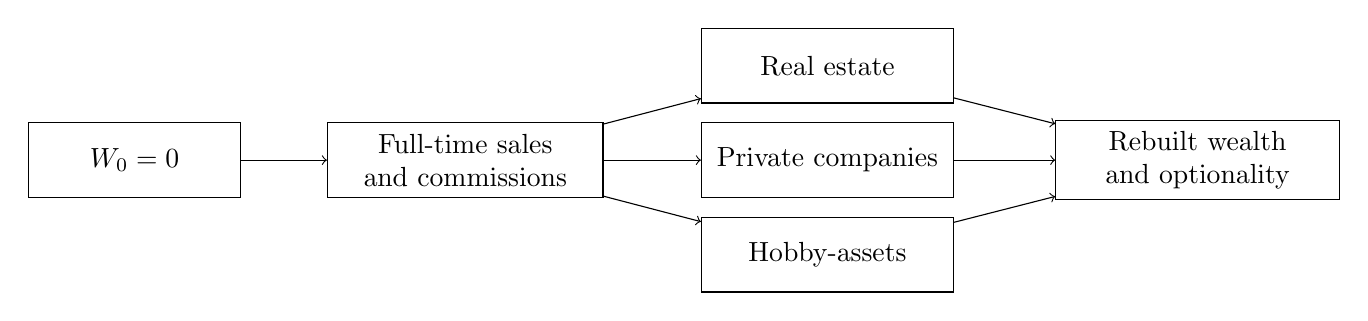
\begin{tikzpicture}[x=1cm,y=1cm]
\node[draw, rectangle, minimum width=2.7cm, minimum height=0.95cm, align=center] (a) at (0,0) {\(W_0=0\)};
\node[draw, rectangle, minimum width=3.5cm, minimum height=0.95cm, align=center] (b) at (4.2,0) {Full-time sales\\and commissions};
\node[draw, rectangle, minimum width=3.2cm, minimum height=0.95cm, align=center] (c) at (8.8,1.2) {Real estate};
\node[draw, rectangle, minimum width=3.2cm, minimum height=0.95cm, align=center] (d) at (8.8,0) {Private companies};
\node[draw, rectangle, minimum width=3.2cm, minimum height=0.95cm, align=center] (e) at (8.8,-1.2) {Hobby-assets};
\node[draw, rectangle, minimum width=3.6cm, minimum height=1cm, align=center] (f) at (13.5,0) {Rebuilt wealth\\and optionality};
\draw[->] (a) -- (b);
\draw[->] (b) -- (c);
\draw[->] (b) -- (d);
\draw[->] (b) -- (e);
\draw[->] (c) -- (f);
\draw[->] (d) -- (f);
\draw[->] (e) -- (f);
\end{tikzpicture}
\end{figure}

The interview then asks what company he would start if he had to begin again. His answer is revealing: the money would not be the hard part now, because he knows enough people to raise it. The idea he would keep in reserve is a company that teaches people how to be better parents. This is not an accidental flourish at the end. It is the commercial reflection of his own value hierarchy. If family really is the first good, then a business devoted to better parenting is not soft sentimentality. It is an investment in the foundation from which later lives are built.

The final question asks how he wants to be remembered. His answer is concise and fitting: as an authentic, hard-working family man who also succeeded in business. After that, the interview returns briefly to the concrete present. Mike describes Virtus as the opposite of a stale industry --- young, energetic, specialized --- with its headquarters in Kansas City and offices in Fort Collins, Chicago, St.~Louis, Austin, Fort Worth, and Memphis, and with over one hundred people. The coda is not accidental. It shows how the interview's larger principles reappear inside a real firm: energy over stagnation, specialization over vagueness, and team over inertia.

\section{Summary}

The interview begins with a viral one-line answer and ends with a compact philosophy of work and life. Along the way it gives us a coherent commercial structure. Career capital compounds through time, execution, and proximity to the right people. Wealth grows not by income alone, but by what is done with income once it arrives. Analytics matters because it converts data into decision-relevant signals. Sales becomes stronger when it is organized as a team of specialists rather than as a collection of isolated generalists. Family, habits, and solitude are not side themes; they are part of the operating conditions that make good judgment and durable performance possible. And when the interview finally asks what survives after titles and bank balances are stripped away, the answer is not obscure: work hard, be a real teammate, make room to think, rebuild motion first, and let legacy become the later objective.